%%%%%%%%%%%%%%%%%%%% author.tex %%%%%%%%%%%%%%%%%%%%%%%%%%%%%%%%%%%
%
% sample root file for your "contribution" to a contributed volume
%
% Use this file as a template for your own input.
%
%%%%%%%%%%%%%%%% Springer %%%%%%%%%%%%%%%%%%%%%%%%%%%%%%%%%%%%%%%%%


% RECOMMENDED %%%%%%%%%%%%%%%%%%%%%%%%%%%%%%%%%%%%%%%%%%%%%%%%%%%
\documentclass{svmult}
%
%% choose options for [] as required from the list
%% in the Reference Guide
%
\usepackage{mathptmx}       % selects Times Roman as basic font
\usepackage{helvet}         % selects Helvetica as sans-serif font
\usepackage{courier}        % selects Courier as typewriter font
\usepackage{type1cm}        % activate if the above 3 fonts are
                             % not available on your system
%
\usepackage{makeidx}         % allows index generation
\usepackage{graphicx}        % standard LaTeX graphics tool
%                             % when including figure files
\usepackage{multicol}        % used for the two-column index
\usepackage[bottom]{footmisc}% places footnotes at page bottom


\usepackage{wrapfig}
\usepackage[caption=false]{subfig}

%\captionsetup{compatibility=false}

%
%% see the list of further useful packages
%% in the Reference Guide
%
%\makeindex             % used for the subject index
%                       % please use the style svind.ist with
%                       % your makeindex program
%
%%%%%%%%%%%%%%%%%%%%%%%%%%%%%%%%%%%%%%%%%%%%%%%%%%%%%%%%%%%%%%%%%%%%%%%%%%%%%%%%%%%%%%%%%%
%
\begin{document}


\title*{Partridge: An effective system for the automatic classification of the types of academic papers}
\titlerunning{Partridge: A system for classification of academic papers}
% Use \titlerunning{Short Title} for an abbreviated version of
% your contribution title if the original one is too long
%\author{James Ravenscroft\,$^{1}$\footnote{to whom correspondence should be addressed}, Maria Liakata\,$^{2,3}$ and Amanda Clare$^{1}$}
%\address{$^{1}$Department of Computer Science, Aberystwyth University,
%$^{2}$Department of Computer Science, University of Warwick,
%$^{2}$Text mining group, EMBL-EBI Cambridge}
\author{James Ravenscroft \and Maria Liakata \and Amanda Clare}
% Use \authorrunning{Short Title} for an abbreviated version of
% your contribution title if the original one is too long
\institute{James Ravenscroft, Amanda Clare \at Department of Computer Science, Aberystwyth University, Aberystwyth, SY23 3DB, UK  \email{ravenscroft@papro.org.uk}, \email{afc@aber.ac.uk}
\and Maria Liakata \at Department of Computer Science, University of Warwick \email{M.Liakata@warwick.ac.uk}}

%
% Use the package "url.sty" to avoid
% problems with special characters
% used in your e-mail or web address
%
\maketitle

\abstract{Partridge is a system that enables intelligent search for
  academic papers by allowing users to query terms within
  sentences designating a particular core scientific concept (e.g. Hypothesis, Result, etc). 
  The system also automatically classifies papers according to
  article types (e.g. Review, Case Study). Here, we focus on the latter
  aspect of the system. For each paper, Partridge automatically
  extracts the full paper content from PDF files, converts it to XML,
  determines sentence boundaries, automatically labels the sentences
  with core scientific concepts, and then uses a random forest model to
  classify the paper type. We show that the type of a paper can be
  reliably predicted by a model which analyses the distribution of
  core scientific concepts within the sentences of the paper. We
  discuss the appropriateness of many of the existing paper types used
  by major journals, and their corresponding distributions. Partridge
  is online and available for use, includes a browser-friendly
  bookmarklet for new paper submission, and demonstrates a range of
  possibilities for more intelligent search in the scientific
  literature. The Partridge instance and further information about
  the project can be found at \url{http://papro.org.uk}}

\section{Introduction} \label{sec:1}

Since the advent of the `Digital Age', the amount of information available to
researchers has been increasing drastically, relevant material is becoming
progressively more difficult to find manually and the need for an automated
information retrieval tool more apparent. There are already a large number of
information retrieval and recommendation systems for scientific publications.
Many of these systems, such as
AGRICOLA\footnote{\url{http://agricola.nal.usda.gov/}}, the Cochrane
Library\footnote{\url{http://www.thecochranelibrary.com/}} and
Textpresso\footnote{\url{http://www.textpresso.org/}} index only publications
from predefined journals or topics (for the above examples, Agriculture,
Biology and Bioinformatics respectively).  Unfortunately, these domain specific
indexing systems usually only contain a small subset of papers, excluding
potentially crucial literature because it does not quite fit into the subject
domain. 

The value of these systems to their users is often restricted by the small
proportion of available literature that they index, forcing researchers to use
multiple, domain specific, search engines for their queries.  In contrast,
there are also a number of interdisciplinary indexing systems and online
journals such as arXiv\footnote{\url{http://arxiv.org}} and
PloSOne\footnote{\url{http://plosone.org}} that try to incorporate wide ranges
of papers from as many disciplines as possible. The traits of these systems
often complement those of their domain-specific counterparts; they provide a
comprehensive collection of literature but insufficient filtering and indexing
capabilities, usually based on title and abstract. 

However, the document title is just one of the crucial parts of a scientific
paper's structure.  Liakata \emph{et al.} (2012) describe a system for
automatically processing and classifying sentences in a research paper
according to the core scientific concept (CoreSC) that they describe
\cite{Liakata2012}.  There are 11 CoreSCs, including {\em Hypothesis}, {\em
Goal}, {\it Background}, {\em Method}, {\em Result} and {\em Conclusion}.
CoreSC labels can be allocated to all sentences in a scientific paper in order
to identify which scientific concept each sentence encapsulates.
SAPIENTA\footnote{\url{http://www.sapientaproject.com}} is a publicly available
machine learning application which can automatically annotate all sentences in
a scientific paper with their CoreSC labels. It was trained using a corpus of
physical chemistry and biochemistry research papers whose sentences were
manually annotated using the CoreSC \cite{LIAKATA10.644} scheme.  An
intelligent information retrieval system can use this data to provide better
filtering and search capabilities for researchers.  Partridge implements such
context-aware keyword search, by allowing researchers to search for papers
where a term appears in sentences with a specific CoreSC label (e.g only in
{\em Method} sentences). This can be used to greatly improve both the precision
with which researchers are able to perform searches for scientific literature
and the accuracy of those searches in terms of relevance to the reader.

The type of a paper ({\em Review}, {\em Case Study}, {\em Research}, {\em
Perspective}, etc) is another useful feature through which a user can narrow
down the results of a search.  The type of a paper can then be used to augment
queries.  For example, a user may search for a {\em Review} paper containing
the keywords ``PCR microfluidics'', or a {\em Research} paper with a {\em
Hypothesis} containing the keywords ``cerevisiae'' and ``glucose''.   Such
paper types are not yet standardised by journals.  We expect the structure of a
paper to reflect its paper type.  For example, review papers would be expected
to contain a large amount of background material.  In this article, we describe
the application of machine learning (using random forests) to create predictive
models of a paper's type, using the distribution of CoreSC labels found in the
full text of the paper. 

This model of paper type is currently in use in our Partridge system, which has
been created as an intelligent full-text search platform for scientific papers.
Partridge (which currently holds 1288 papers and is constantly expanding) 
makes use of automatically derived CoreSC sentence labels and
automatically derived paper types, to allow deeper information queries.  We
discuss the reliability of this model of paper types and the insights that have
been gained for the authorship of papers.


\section{Methods}
\label{sec:2}
%how types were chosen,

\subsection{Collection of scientific articles} 
Partridge allows users to upload any paper which is free of copyright
restrictions.  For the purpose of this study we needed a large set of papers
that we could label with CoreSC to investigate how this information assists
classification into paper type.  Open Access (OA) journals provide free read
access to their papers, but many do not permit the user of articles for data
mining purposes. The Public Library of Science (PLoS) journals contain large
volumes of OA literature under a permissive license that allows data mining.
They also use the PubMed Central markup schema, which is compatible with
SAPIENTA, for papers published through their journal. The PLoS journals
advanced search offers approximately 50 types of paper through which to
restrict the search.  Many of these paper type categories contain too few
papers to be useful, others are too ad hoc (e.g.  {\it Message from PLoS}).
Indeed it is not clear how these paper types have been identified. We chose to
look at a range of types, some of which we expect to overlap or have an unclear
distinction.  These are namely: Essay, Correspondence, Case Study, Perspective,
Viewpoint, Opinion, Review, Research. 

% in conclusions add how this can give recommendations for Plos and other
% journals 
A script called {\em plosget.py}\footnote{\url{https://github.com/ravenscroftj/partridge}} was written, in order to download the
papers via the PloS RESTful search API\footnote{\url{http://api.plos.org/solr/faq/}}. The number of papers downloaded per
paper type category was as follows: 200 Essay, 99 Correspondence, 107 Case
Study, 200 Perspective, 74 Viewpoint, 93 Opinion, 312 Review, 200 Research.
These formed a corpus of 1285 %1459-174 after removing synopsis. Should double
check the numbers add up papers.

Figure \ref{fig:coresc_pies} shows the CoreSC content of a review paper and a
research paper randomly selected from the corpus.  The review papers tend to be
made up almost entirely from Background CoreSC sentences.  However, research
papers are much more evenly spread, made up of several different types of
CoreSC.  This investigation suggested that there is almost certainly a
discriminative relationship between CoreSC categories and a paper's type. 



\begin{figure}[t]
\centering
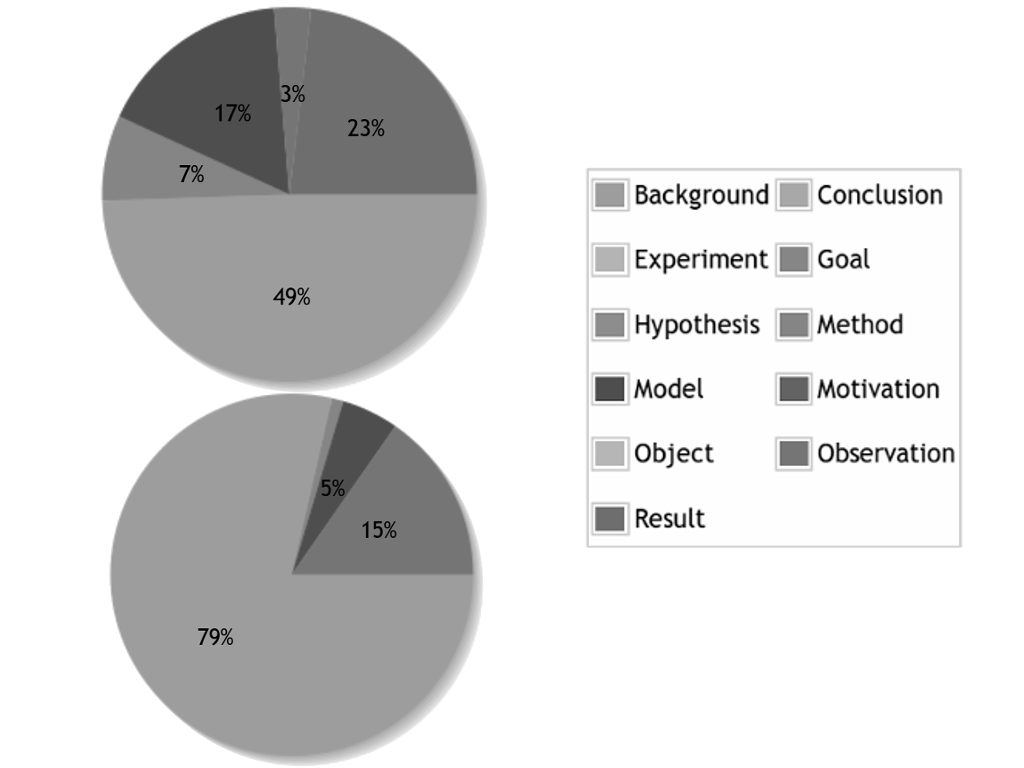
\includegraphics[width=\textwidth]{figures/corescs.png}
\caption{The CoreSC makeup of a research paper and a review paper randomly selected from the corpus}
\label{fig:coresc_pies} 
\end{figure}

\subsection{Paper Processing and Classification}
%Discuss in more detail how Partridge processes papers (PDFX, sentence splitting) 

In order to obtain automatic labeling of sentences in a paper with CoreSC
concepts we first needed to convert the papers to a format that the the CoreSC
classifier, SAPIENTA can analyse.  Currently, SAPIENTA supports the SciXML and
PubMed Central DTDs.  Papers in PDF format are first converted to XML using
PDFX , a free service hosted by the University of Manchester
\cite{Constantin2013}. Once the paper has been split into sentences with
Liakata's SSplit tool \cite{liakata2009semantic}, SAPIENTA is used to annotate
each sentence with a relevant CoreSC label. These labels are assigned using a
conditional random fields model based upon a number of features such as the
sentence's location within the paper and pairs and triplets of words found
consecutively within the sentence \cite{Liakata2012}.  The SAPIENTA system has
been trained on a corpus of 265 chemistry and biochemistry papers and we have
done no domain adaptation for the papers in PLoS.


%how the machine learning is conducted (random forest using orange, features, validation methods).

Random forest learning \cite{Breiman2001} was chosen for the construction of the
paper type classifier. This is because random forests are a fast, accurate and
widely accepted learning technology, and the underlying decision trees can be
inspected to understand some of the reasoning behind the predictions made by
the final paper type classifiers. The feature set consisted of the percentage
composition of each of the 11 respective CoreSC labels assigned to the
sentences in each paper i.e. (the percentage of {\em Background} sentences, the
percentage of {\em Hypothesis} sentences, etc.). The random forest learning was
conducted using the Orange data mining library for Python \cite{Curk2005}.  The
parameters for the random forest learner were as the defaults, except with
min\_subsets=5 and same\_majority\_pruning=true.  We used 10-fold cross
validation to estimate the precision, recall and F-measure.


\section{Results and Discussion}
\label{sec:3}


\begin{table}

\caption{Per-class recall, precision and F-measure micro-averaged over 10-fold cross validation, reporting the results on the held-out validation segment. Top paper types in bold.}

\begin{tabular}{p{2.4cm}p{2.0cm}p{2.0cm}p{2.5cm}}
\hline\noalign{\smallskip}
Classes & Recall(\verb|%|) & Precision(\verb|%|)& F-measure(\verb|%|) \\
\noalign{\smallskip}\svhline\noalign{\smallskip}
Case Study      &   24.3    &    24.5     &   24.4 \\
Correspondence  &   {\bf  54.5}    &    {\bf 50.5}    &    {\bf 52.4} \\ 
Essay           &   45.0     &   46.2    &    45.6 \\
Opinion         &   24.7    &    23.5  &      24.1 \\   
Perspective     &   25.5  &      30.4  &       27.7 \\
Research        &   {\bf 70.0}    &    {\bf 61.9}    &    {\bf 65.7} \\
Review          &  {\bf 63.1}     &   {\bf 62.5}     &   {\bf 62.8} \\
Viewpoint       &     14.9     &   15.7  &      15.3 \\
\noalign{\smallskip}\hline\noalign{\smallskip}
\end{tabular}


\label{tab:recallPrecision}       % Give a unique label
\end{table}

The results of the random forest learning as recall, precision and F-measure
for each paper type, averaged over a 10-fold cross validation are shown in Table
\ref{tab:recallPrecision}. Paper types {\em Research}, {\em Review} and {\em
Correspondence} are the most accurate classes, and {\em Viewpoint} is the most
difficult paper type to predict. 


A confusion matrix for the paper types is given in Table
\ref{tab:confusion}. Research papers are usually predicted to belong
to the Research class, and are sometimes confused with Case
Study. However, Case Study papers are often predicted to be Research
or Review. The ratio between Case Study, Research and Review papers is
~1:2:3 so the outcome is not entirely surprising in terms of the data
size effect. We expected Research and Case Study to share similar
paper structures but perhaps the fact that Case Study is equally
confused with Research and Review suggests two distinct types of Case
Study.  We expected the classes Essay, Opinion, Perspective and
Viewpoint to be confused, as the four labels all indicate a paper
containing an author's personal thoughts on an issue, rather than
experiment-driven science. Opinion is confused with Perspective and
Viewpoint. Perspective is confused with almost all classes, except
Research. Viewpoint is a small class and mostly confused with Opinion
and Perspective. From this it would seem that the paper types
\{Opinion, Perspective, Viewpoint\} are very similar and should be
grouped together into one category. Indeed when we trained the model
on a super class consisting of the previous three categories,
performance was improved overall with the following F-measures:
OpinionSuper: 59, Research: 67.6, Review: 63.7, Essay: 44.9,
Correspondence: 46 and Case Study 24.8.

\begin{table}

\caption{Confusion matrix summed over 10-fold cross validation, reporting the results on the held-out validation segment. Rows represent true classes, columns represent predicted classes.}
\label{tab:confusion}       % Give a unique label]

\begin{tabular}{lllllllll}
\hline\noalign{\smallskip}
      &  Case Study   &     Corresp.      &   Essay  & Opinion &     Perspective    &     Research    &     Review  & Viewpoint \\
\noalign{\smallskip}\svhline\noalign{\smallskip}
Case Study    &    26   &     2     &   11    &    2  &      5 & 26       & 25 &       10 \\
Correspondence  &      4  &      54   &     3    &    9     &   15 & 8   &     4 &       2 \\
Essay      &  8     &   5    &   90    &    2 &       39      &  5 & 46    &    5 \\
Opinion    &    4   &     7 &       2   &     23      &  27     &   10   &  3  &      17 \\
Perspective &       11  &      16    &    49       & 30      &  51 & 6      &  26    &   11 \\
Research      &  19    &    6 &       2 &       8    &    5      &  140  &   12    &    8\\
Review       & 27     &   8     &   35    &    5      &  13    &    21   &  197 &       6\\
Viewpoint    &    7  &      9   &     3     &   19     &   13 & 10     &   2  &      11 \\
\noalign{\smallskip}\hline\noalign{\smallskip}
\end{tabular}
\end{table}



%Discuss why it's possible to predict type from CoreSC (which CoreSC define a class).

We inspected the detail of a single decision tree, grown on the entire dataset,
to gain further insight into which CoreSC class decisions were responsible for
the paper type predictions. This was a very large tree, with a depth of 37
nodes in places.  The first decision was based upon the number of Background
sentences in the article. Low Background percentages, of less than 0.694
indicates a Correspondence paper. 28 out of the 31 Correspondence papers were
correctly classified by this decision.

The next decision, for higher amounts of Background, was based on the
percentage of Experiment sentences in the paper. For a very low
percentage of Experiment sentences ($<$ 0.061), the papers then
branched into a long side chain of detailed classification decisions,
to separate mostly the Opinion, Viewpoint and Perspective papers from
other Correspondence papers, and a few examples of the remaining
categories. For a higher percentage of Experiment sentences, Research
papers were classified as those that had Observations $>$ 5.6\%, or
Conclusions $<=$ 1.4\%, whereas Case Studies had fewer Observations
and more Conclusions.

The largest node classifying Essay did so via a route after the low
Experiment decision that asked for a Background $>$ 48\%, but then low
values for Goal, Hypothesis, Result, Observation, Model, Conclusion
and Object. These decisions seem reasonable and agreed with our
expectations of the content of an Essay.

\section{Summary and Conclusions}
\label{sec:4}
To summarise, we have demonstrated that paper type can largely be predicted
from the distribution of the automatically obtained CoreSC sentence labels in
the full text of a paper. We have described some of the particular CoreSC
features that determine a paper type (e.g. Correspondence characterised by very
little Background, Opinions characterised by low percentage of Experiment) and
discussed which of the paper types are not easily separable in this way. We
recommended for example merging the Opinion, Viewpoint and Perspective articles
into a single category, which increased overall classification performance. It
is also potentially useful to distinguish between two types of Case study.
Analysis of an example tree shows the decision making process to be complex,
but agrees with our general understanding of paper types. Partridge allows refinement of paper search using CoreSC and paper type, both of which
can be intelligently determined using machine learning methods.


%Discuss the potential for intelligent paper search opportunities in general and the future for Partridge.

The potential for automatic extraction of useful features from
scientific papers to assist researchers in their knowledge queries is
now an exciting area for research. Open Access journals that permit
full text mining lead the way in allowing this research to expand and
flourish. In future work we aim to develop and implement a range of
further useful properties that will uncover more of the information
that is hidden within the text of articles, and to use Partridge as a
working engine to demonstrate their usefulness in practice.

\begin{acknowledgement} We thank the Leverhulme Trust for the support to Dr
Liakata's Early Career Fellowship and also EMBL-EBI, Cambridge UK for the
facilities offered to Dr Liakata.  \end{acknowledgement}

\bibliographystyle{spphys}
\bibliography{partridge}

%%%%%%%%%%%%%%%%%%%%%%%%% referenc.tex %%%%%%%%%%%%%%%%%%%%%
% sample references
% 
% Use this file as a template for your own input.
%
%%%%%%%%%%%%%%%%%%%%%%%% Springer%%%%%%%%%%%%%%%%%%%%%%%%%%
%
% BibTeX users please use
% \bibliographystyle{}
% \bibliography{}
%
\biblstarthook{References may be \textit{cited} in the text either by number (preferred) or by author/year.\footnote{Make sure that all references from the list are cited in the text. Those not cited should be moved to a separate \textit{Further Reading} section or chapter.} The reference list should ideally be \textit{sorted} in alphabetical order -- even if reference numbers are used for the their citation in the text. If there are several works by the same author, the following order should be used: 
\begin{enumerate}
\item all works by the author alone, ordered chronologically by year of publication
\item all works by the author with a coauthor, ordered alphabetically by coauthor
\item all works by the author with several coauthors, ordered chronologically by year of publication.
\end{enumerate}
The \textit{styling} of references\footnote{Always use the standard abbreviation of a journal's name according to the ISSN \textit{List of Title Word Abbreviations}, see \url{http://www.issn.org/en/node/344}} depends on the subject of your book:
\begin{itemize}
\item The \textit{two} recommended styles for references in books on \textit{mathematical, physical, statistical and computer sciences} are depicted in ~\cite{science-contrib, science-online, science-mono, science-journal, science-DOI} and ~\cite{phys-online, phys-mono, phys-journal, phys-DOI, phys-contrib}.
\item Examples of the most commonly used reference style in books on \textit{Psychology, Social Sciences} are~\cite{psysoc-mono, psysoc-online,psysoc-journal, psysoc-contrib, psysoc-DOI}.
\item Examples for references in books on \textit{Humanities, Linguistics, Philosophy} are~\cite{humlinphil-journal, humlinphil-contrib, humlinphil-mono, humlinphil-online, humlinphil-DOI}.
\item Examples of the basic Springer style used in publications on a wide range of subjects such as \textit{Computer Science, Economics, Engineering, Geosciences, Life Sciences, Medicine, Biomedicine} are ~\cite{basic-contrib, basic-online, basic-journal, basic-DOI, basic-mono}. 
\end{itemize}
}

\begin{thebibliography}{99.}%
% and use \bibitem to create references.
%
% Use the following syntax and markup for your references if 
% the subject of your book is from the field 
% "Mathematics, Physics, Statistics, Computer Science"
%
% Contribution 
\bibitem{science-contrib} Broy, M.: Software engineering --- from auxiliary to key technologies. In: Broy, M., Dener, E. (eds.) Software Pioneers, pp. 10-13. Springer, Heidelberg (2002)
%
% Online Document
\bibitem{science-online} Dod, J.: Effective substances. In: The Dictionary of Substances and Their Effects. Royal Society of Chemistry (1999) Available via DIALOG. \\
\url{http://www.rsc.org/dose/title of subordinate document. Cited 15 Jan 1999}
%
% Monograph
\bibitem{science-mono} Geddes, K.O., Czapor, S.R., Labahn, G.: Algorithms for Computer Algebra. Kluwer, Boston (1992) 
%
% Journal article
\bibitem{science-journal} Hamburger, C.: Quasimonotonicity, regularity and duality for nonlinear systems of partial differential equations. Ann. Mat. Pura. Appl. \textbf{169}, 321--354 (1995)
%
% Journal article by DOI
\bibitem{science-DOI} Slifka, M.K., Whitton, J.L.: Clinical implications of dysregulated cytokine production. J. Mol. Med. (2000) doi: 10.1007/s001090000086 
%
\bigskip

% Use the following (APS) syntax and markup for your references if 
% the subject of your book is from the field 
% "Mathematics, Physics, Statistics, Computer Science"
%
% Online Document
\bibitem{phys-online} J. Dod, in \textit{The Dictionary of Substances and Their Effects}, Royal Society of Chemistry. (Available via DIALOG, 1999), 
\url{http://www.rsc.org/dose/title of subordinate document. Cited 15 Jan 1999}
%
% Monograph
\bibitem{phys-mono} H. Ibach, H. L\"uth, \textit{Solid-State Physics}, 2nd edn. (Springer, New York, 1996), pp. 45-56 
%
% Journal article
\bibitem{phys-journal} S. Preuss, A. Demchuk Jr., M. Stuke, Appl. Phys. A \textbf{61}
%
% Journal article by DOI
\bibitem{phys-DOI} M.K. Slifka, J.L. Whitton, J. Mol. Med., doi: 10.1007/s001090000086
%
% Contribution 
\bibitem{phys-contrib} S.E. Smith, in \textit{Neuromuscular Junction}, ed. by E. Zaimis. Handbook of Experimental Pharmacology, vol 42 (Springer, Heidelberg, 1976), p. 593
%
\bigskip
%
% Use the following syntax and markup for your references if 
% the subject of your book is from the field 
% "Psychology, Social Sciences"
%
%
% Monograph
\bibitem{psysoc-mono} Calfee, R.~C., \& Valencia, R.~R. (1991). \textit{APA guide to preparing manuscripts for journal publication.} Washington, DC: American Psychological Association.
%
% Online Document
\bibitem{psysoc-online} Dod, J. (1999). Effective substances. In: The dictionary of substances and their effects. Royal Society of Chemistry. Available via DIALOG. \\
\url{http://www.rsc.org/dose/Effective substances.} Cited 15 Jan 1999.
%
% Journal article
\bibitem{psysoc-journal} Harris, M., Karper, E., Stacks, G., Hoffman, D., DeNiro, R., Cruz, P., et al. (2001). Writing labs and the Hollywood connection. \textit{J Film} Writing, 44(3), 213--245.
%
% Contribution 
\bibitem{psysoc-contrib} O'Neil, J.~M., \& Egan, J. (1992). Men's and women's gender role journeys: Metaphor for healing, transition, and transformation. In B.~R. Wainrig (Ed.), \textit{Gender issues across the life cycle} (pp. 107--123). New York: Springer.
%
% Journal article by DOI
\bibitem{psysoc-DOI}Kreger, M., Brindis, C.D., Manuel, D.M., Sassoubre, L. (2007). Lessons learned in systems change initiatives: benchmarks and indicators. \textit{American Journal of Community Psychology}, doi: 10.1007/s10464-007-9108-14.
%
%
% Use the following syntax and markup for your references if 
% the subject of your book is from the field 
% "Humanities, Linguistics, Philosophy"
%
\bigskip
%
% Journal article
\bibitem{humlinphil-journal} Alber John, Daniel C. O'Connell, and Sabine Kowal. 2002. Personal perspective in TV interviews. \textit{Pragmatics} 12:257--271
%
% Contribution 
\bibitem{humlinphil-contrib} Cameron, Deborah. 1997. Theoretical debates in feminist linguistics: Questions of sex and gender. In \textit{Gender and discourse}, ed. Ruth Wodak, 99--119. London: Sage Publications.
%
% Monograph
\bibitem{humlinphil-mono} Cameron, Deborah. 1985. \textit{Feminism and linguistic theory.} New York: St. Martin's Press.
%
% Online Document
\bibitem{humlinphil-online} Dod, Jake. 1999. Effective substances. In: The dictionary of substances and their effects. Royal Society of Chemistry. Available via DIALOG. \\
http://www.rsc.org/dose/title of subordinate document. Cited 15 Jan 1999
%
% Journal article by DOI
\bibitem{humlinphil-DOI} Suleiman, Camelia, Daniel C. O�Connell, and Sabine Kowal. 2002. `If you and I, if we, in this later day, lose that sacred fire...�': Perspective in political interviews. \textit{Journal of Psycholinguistic Research}. doi: 10.1023/A:1015592129296.
%
%
%
\bigskip
%
%
% Use the following syntax and markup for your references if 
% the subject of your book is from the field 
% "Computer Science, Economics, Engineering, Geosciences, Life Sciences"
%
%
% Contribution 
\bibitem{basic-contrib} Brown B, Aaron M (2001) The politics of nature. In: Smith J (ed) The rise of modern genomics, 3rd edn. Wiley, New York 
%
% Online Document
\bibitem{basic-online} Dod J (1999) Effective Substances. In: The dictionary of substances and their effects. Royal Society of Chemistry. Available via DIALOG. \\
\url{http://www.rsc.org/dose/title of subordinate document. Cited 15 Jan 1999}
%
% Journal article by DOI
\bibitem{basic-DOI} Slifka MK, Whitton JL (2000) Clinical implications of dysregulated cytokine production. J Mol Med, doi: 10.1007/s001090000086
%
% Journal article
\bibitem{basic-journal} Smith J, Jones M Jr, Houghton L et al (1999) Future of health insurance. N Engl J Med 965:325--329
%
% Monograph
\bibitem{basic-mono} South J, Blass B (2001) The future of modern genomics. Blackwell, London 
%
\end{thebibliography}

\end{document}
